\section{Νευρωνικά Δίκτυα Συνέλιξης}
\label{sec:theory_cnn}

Έως τώρα μιλήσαμε για τα πολυεπίπεδα νευρωνικά δίκτυα και την γενικότερη
λειτουργία τους. Σε αυτό το υποκεφάλαιο θα μιλήσουμε για συγκεκριμένα μοντέλα
πολυεπίπεδων νευρωνικών δικτύων και πιο συγκεκριμένα για τα
\emph{Νευρωνικά Δίκτυα Συνέλιξης}. Τα συγκεκριμένα μοντέλα χρησιμοποιούνται
σήμερα κυρίως στα προβλήματα της αναγνώρισης και εντοπισμού αντικειμένων
σε εικόνες.

Ο τρόπος λειτουργίας τους είναι όμοιος με αυτόν που παρουσιάστηκε στο % το ; είναι ελληνικό ερωτηματικό, στα αγγλικά είναι άνω τελεία.
\autoref{sec:theory_dnn}; αποτελούνται από πολλά επίπεδα, όπου το κάθε επίπεδο αποτελείται
από έναν αριθμό νευρώνων οι οποίοι έχουν σαν παραμέτρους εκμάθησης τα βάρη τους ($w_{\jmath}^{\imath}$)
και την τιμή πόλωσης ($b^{\imath}$).
Κάθε νευρώνας δέχεται ένα σήμα εισόδου, εφαρμόζει μία πράξη εσωτερικού γινομένου σε αυτό,
και προαιρετικά εφαρμόζει στο αποτέλεσμα μία μη γραμμική συνάρτηση.
Το τελευταίο επίπεδο των CNN είναι πλήρες συνδεδεμένο και έχει μία
συνάρτηση σφάλματος.
Η διαφορά των μοντέλων CNN από τα κλασσικά ANN είναι ότι θεωρούν για δεδομένα εισόδου
εικόνες.

Αυτό που καταφέρνουν να κάνουν τα CNN είναι να μοντελοποιήσουν μικρά
τμήματα πληροφορίας, τα οποία στην συνέχεια ενώνονται για να δημιουργήσουν
υψηλότερου επιπέδου πληροφορία. Αν για παράδειγμα παρατηρήσουμε την λειτουργία
ενός μοντέλου CNN, το πρώτο επίπεδο προσπαθεί να εντοπίσει ακμές, το δεύτερο
επίπεδο παίρνει την πληροφορία των ακμών και προσπαθεί να εντοπίσει περιγράμματα,
κτλ.

Σε κάθε εικονοστοιχείο της εικόνας αντιστοιχούν 3 τιμές (RGB) και άρα η είσοδος σε ένα
CNN έχει τρεις διαστάσεις όπως φαίνεται και στο \autoref{fig:cnn_1}.
Για παράδειγμα ένα CNN το οποίο έχει σχεδιαστεί να δέχεται σαν είσοδο εικόνες ανάλυσης $80\times60$
έχει επίπεδο εισόδου διαστάσεων $80\times60\times3$.

\begin{figure}[!ht]
  \centering
  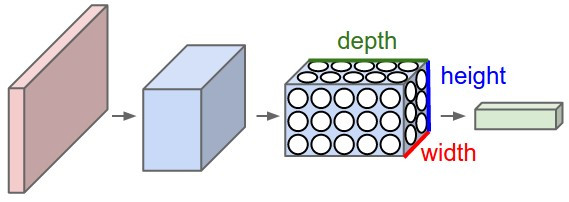
\includegraphics[width=0.8\textwidth]{./images/chapter3/cnn.jpg}
  \caption[Τρισδιάστατη κατανομή των νευρώνων στα CNN]{Τρισδιάστατη κατανομή των νευρώνων στα CNN}
  \label{fig:cnn_1}
\end{figure}

Κάθε επίπεδο ενός CNN παίρνει σαν είσοδο μία μορφή όγκου την οποία
και μετασχηματίζει σε μία άλλη μορφή όγκου.

Οι τρεις βασικοί τύποι επιπέδων που χρησιμοποιούνται σε αρχιτεκτονικές CNN είναι:
\begin{itemize}
  \item{Επίπεδο Συνέλιξης - Convolutional Layer (CONV)}
  \item{Επίπεδο Υπόδειγματοληψίας- Pooling Layer (POOL)}
  \item{Πλήρως Συνδεδεμένο Επίπεδο - Fully-Connected Layer (FC)}
\end{itemize}
Μία σημαντική παρατήρηση είναι ότι τα επίπεδα CONV και FC έχουν παραμέτρους, δηλαδή
βάρη και τιμή πόλωσης των νευρώνων, ενώ τα επίπεδα POOL εκτελούν λειτουργία
δειγματοληψίας στα δεδομένα εισόδου τους.

\subsection{Επίπεδο Συνέλιξης}

Τα επίπεδα συνέλιξης είναι ο πυρήνας των μοντέλων CNN. Οι παράμετροι ενός
επιπέδου CONV είναι μία σειρά από δισδιάστατα φίλτρα τα οποία όμως εκτείνονται
σε όλο το σε όλο το βάθος του όγκου εισόδου. Το βάθος των φίλτρων αυτών
ισούται με το βάθος του όγκου στην είσοδο.

Όπως αναφέραμε και προηγουμένως, τα επίπεδα CONV εφαρμόζουν πράξη συνέλιξης πάνω στα
δεδομένα εισόδου. Αυτό επηρρεάζει την δομή των "τοπικών" διασυνδέσεων.
Στο παράδειγμα του σχήματος \ref{fig:cnn_2} βλέπουμε πως ο κάθε νευρώνας
του επιπέδου συνέλιξης συνδέεται με μία περιοχή του όγκου στην είσοδό του.

\begin{figure}[!ht]
  \centering
  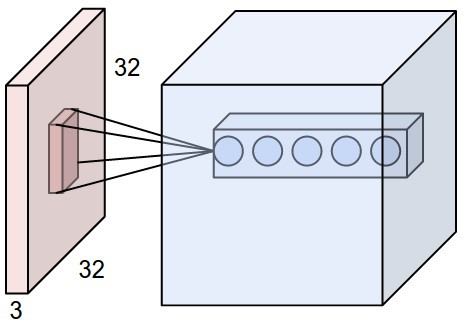
\includegraphics[width=0.4\textwidth]{./images/chapter3/cnn_2.jpg}
  \caption[%
    Παράδειγμα διασύνδεσης τρισδιάστατης εισόδου με την τρισδιάστατη δομή των
    νευρόνων ενός επιπέδου συνέλιξης (CONV)]{%
    Παράδειγμα διασύνδεσης τρισδιάστατης εισόδου με την τρισδιάστατη δομή των
    νευρόνων ενός επιπέδου συνέλιξης (CONV)}
  \label{fig:cnn_2}
\end{figure}

Η συνέλιξη ενός φίλτρου με τον τον όγκο εισόδου παράγει έναν \emph{χάρτη ενεργοποίησης (activation map)},
με τον τρόπο που φαίνεται στο \autoref{fig:cnn_activation_map}. Στο παράδειγμα αυτό
εφαρμόζεται φίλτρο διαστάσεων $5\times5\times3$ σε έναν όγκο $32 \times 32 \times 3$ και παράγεται
ένας χάρτης ενεργοποίησης διαστάσεων $28\times28\times1$.

\begin{figure}[!ht]
  \centering
  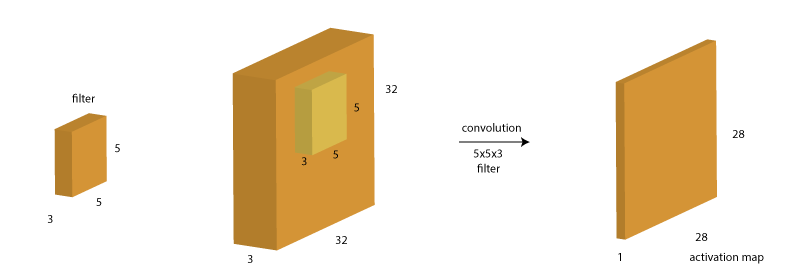
\includegraphics[width=1\textwidth]{./images/chapter3/cnn_activation_map.png}
  \caption[Συνέλιξη φίλτρου ενός επιπέδου συνέλιξης με τον όγκο εισόδου και παραγωγή ενός χάρτη ενεργοποίησης]{Συνέλιξη φίλτρου ενός επιπέδου συνέλιξης με τον όγκο εισόδου και παραγωγή ενός χάρτη ενεργοποίησης}
  \label{fig:cnn_activation_map}
\end{figure}

Η μείωση των διαστάσεων μήκους και πλάτους από $32 \times 32$ σε $28 \times 28$ οφείλεται στον τρόπο με τον οποίο
εκτελείται η πράξη της συνέλιξης των φίλτρων με τον όγκο εισόδου  (\autoref{fig:cnn_conv}).
Οι διαστάσεις του όγκου εξόδου, έχοντας σαν είσοδο όγκο διαστάσεων $N \times N \times d$ και φίλτρων $F \times F \times d$ υπολογίζονται, στην απλούστερη περίπτωση με βάση την σχέση
\begin{equation*}
  outsize = (N-F) + 1
\end{equation*}


\begin{figure}[!ht]
  \centering
  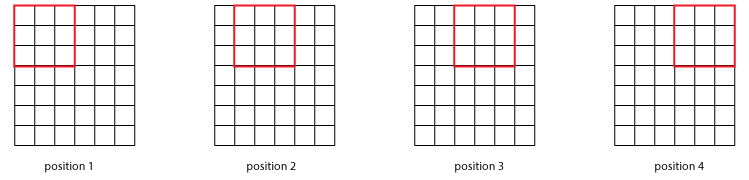
\includegraphics[width=1\textwidth]{./images/chapter3/cnn_conv.png}
  \caption[Διαδικασία Συνέλιξης]{Διαδικασία Συνέλιξης}
  \label{fig:cnn_conv}
\end{figure}

Η τιμή του βάθους του όγκου στην έξοδο ενός επιπέδου CONV αντιστοιχεί στον αριθμό των φίλτρων που
εφαρμόζονται στον όγκο εισόδου. Δηλαδή ο αριθμός των χαρτών ενεργοποίησης
αντιστοιχεί στον αριθμό των φίλτρων. Αν για παράδειγμα ο όγκος εισόδου είναι
διαστάσεων $32 \times 32 \times 3$ και εφαρμόσουμε δέκα φίλτρα συνέλιξης διαστάσεων $5\times5\times3$,
ο όγκος εξόδου θα είναι διαστάσεων $28\times28\times3$ \autoref{fig:cnn_num_filters}.
Ο αριθμός των φίλτρων είναι μία παράμετρος, ή καλύτερα \emph{υπερ-παράμετρος} των επιπέδων συνέλιξης.

\begin{figure}[!ht]
  \centering
  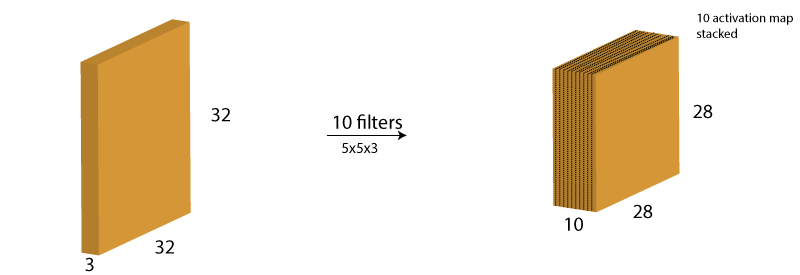
\includegraphics[width=1\textwidth]{./images/chapter3/cnn_num_filters.png}
  \caption[Αντιστοιχία του αριθμού των φίλτρων ενός επιπέδου συνέλιξης με το βάθος του όγκου στην έξοδο]{Αντιστοιχία του αριθμού των φίλτρων ενός επιπέδου συνέλιξης με το βάθος του όγκου στην έξοδο}
  \label{fig:cnn_num_filters}
\end{figure}

Ωστόσο, το βήμα μετατόπισης (stride) του φίλτρου πάνω στην είσοδο είναι και αυτό
μία υπέρ-παράμετρος (hyperparameter) των επιπέδων συνέλιξης.
Χρησιμοποιώντας βήμα μετατόπισης (S) διάφορο της μονάδας καταλήγουμε στην πιο κάτω
εξίσωση για τον υπολογισμό του όγκου εξόδου:
\begin{equation*}
  outsize = (N-F)/S + 1
\end{equation*}

Ένα πρόβλημα που εμφανίζεται στην περίπτωση των μοντέλων CNN με μεγάλο αριθμό
κρυφών επιπέδων είναι η γρήγορη μείωση των διαστάσεων μήκους και πλάτους του
όγκου, το οποίο είναι αποτέλεσμα της διαδοχικής εφαρμογής πράξεων συνέλιξης (\autoref{fig:cnn_shrunk}).

\begin{figure}[!ht]
  \centering
  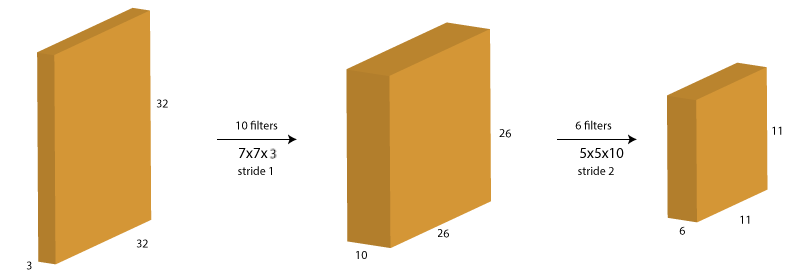
\includegraphics[width=1\textwidth]{./images/chapter3/cnn_shrunk.png}
  \caption[Διαδοχικές εφαρμογές του τελεστή συνέλιξης προκαλούν μείωση των διαστάσεων μήκους και πλάτους του όγκου]{Διαδοχικές εφαρμογές του τελεστή συνέλιξης προκαλούν μείωση των διαστάσεων μήκους και πλάτους του όγκου}
  \label{fig:cnn_shrunk}
\end{figure}

Αυτή η συμπεριφορά είναι ανεπιθύμητη αφού περιορίζει και τις διαστάσεις των φίλτρων
που μπορούμε να χρησιμοποιήσουμε σε κάθε επίπεδο CONV. Η χρήση φίλτρων μεγάλων
διαστάσεων φέρει σαν αποτέλεσμα την γρήγορη μείωση των διαστάσεων του όγκου.

Για να αποτρέψουμε αυτή την συμπεριφορά μπορούμε να επεκτείνουμε τις διαστάσεις
μήκους και πλάτους, προσθέτοντας μηδενικά στα σύνορα του όγκου εισόδου του
εκάστοτε επιπέδου CONV. Η διαδικασία αυτή ονομάζεται
\emph{zero-padding} και φαίνεται στο \autoref{fig:cnn_zero_padding}.
\begin{figure}[!ht]
  \centering
  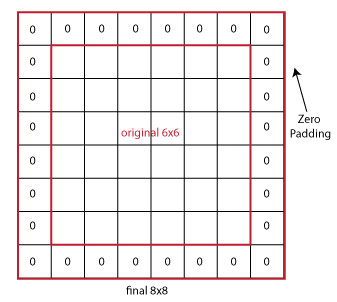
\includegraphics[width=0.6\textwidth]{./images/chapter3/cnn_zero_padding.png}
  \caption[Zero Padding]{Zero Padding}
  \label{fig:cnn_zero_padding}
\end{figure}
Το μέγεθος του συνόρου που προστίθεται είναι η τρίτη υπέρ-παράμετρος ενός
επιπέδου συνέλιξης.

Με την εισαγωγή της υπέρ-παραμέτρου zero-padding η εξίσωση υπολογισμού του όγκου
εξόδου έχει την μορφή:
\begin{equation*}
  outsize = (N - F + 2P)/S + 1
\end{equation*}

Συνοψίζοντας, ένα επίπεδο συνέλιξης έχει τα εξής χαρακτηριστικά:
\begin{itemize}
  \item{Διαστάσεις όγκου εισόδου: $W_{1} \times H_{1} \times D_{1}$}
  \item{Hyperparameters:}
    \begin{itemize}
      \item{K: Αριθμός φίλτρων}
      \item{F: Μέγεθος του φίλτρου ($F \times F$)}
      \item{S: Βήμα μετατόπισης}
      \item{P: Ποσότητα zero-padding}
    \end{itemize}
  \item{Διαστάσεις όγκου εξόδου: $W_{2} \times H_{2} \times D_{2}$, $D_{2} = K$} όπου:
    \begin{itemize}
      \item{$W_{2} = (W_{1} - F)/S + 1$}
      \item{$H_{2} = (H_{1} - F)/S + 1$}
      \item{$D_{2} = D_{1}$}
    \end{itemize}
\end{itemize}


\subsection{Επίπεδο Υπό-δειγματοληψίας - Pooling layer}

Συνήθως τα επίπεδα υπό-δειγματοληψίας προστίθενται στο δίκτυο, μεταξύ διαδοχικών
επιπέδων συνέλιξης. Η λειτουργία τους είναι να μειώσουν τις χωρικές
διαστάσεις των αναπαραστάσεων, μειώνοντας έτσι τον αριθμό των
παραμέτρων και άρα τους υπολογισμούς που γίνονται στο νευρωνικό δίκτυο, ενεργώντας σαν
μία συνάρτηση υποδειγματοληψίας
(\autoref{fig:cnn_pool}).

\begin{figure}[!ht]
  \centering
  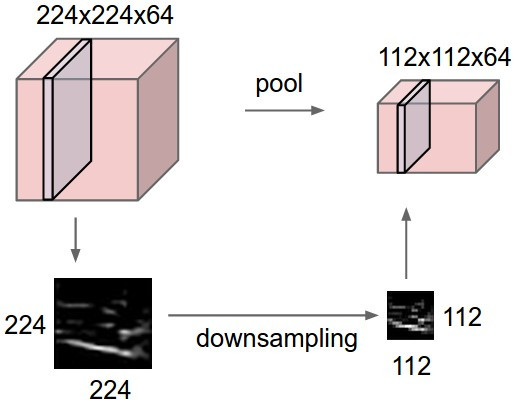
\includegraphics[width=0.6\textwidth]{./images/chapter3/cnn_pool.jpg}
  \caption[Επίπεδο Υποδειγματοληψίας - Pooling layer]{Επίπεδο Υπό-δειγματοληψίας - Pooling layer}
  \label{fig:cnn_pool}
\end{figure}
Πιθανές συναρτήσεις υπό-δειγματοληψίας είναι οι συναρτήσεις \emph{max, average και L2-Norm}

Στο \autoref{fig:cnn_pool_max} βλέπουμε το αποτέλεσμα της εφαρμογής της συνάρτησης
δειγματοληψίας $max(\vec{v})$ πάνω σε ένα πλέγμα διαστάσεων $4 \times 4$.

\begin{figure}[!ht]
  \centering
  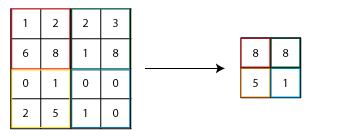
\includegraphics[width=0.6\textwidth]{./images/chapter3/cnn_pool_max.png}
  \caption[Συνάρτηση υπό-δειγματοληψίας Max - Max Pooling]{Συνάρτησης υπό-δειγματοληψίας Max - Max Pooling}
  \label{fig:cnn_pool_max}
\end{figure}

Τα χαρακτηριστικά των συναρτήσεων υπό-δειγματοληψίας είναι:
\begin{itemize}
  \item{Διαστάσεις όγκου εισόδου: $W_{1} \times H_{1} \times D_{1}$}
  \item{Hyperparameters:}
    \begin{itemize}
      \item{F: Χωρική τους έκταση ($F \times F$)}
      \item{S: Βήμα μετατόπισης}
    \end{itemize}
  \item{Διαστάσεις όγκου εξόδου: $W_{2} \times H_{2} \times D_{2}$, $D_{2} = K$} όπου:
    \begin{itemize}
      \item{$W_{2} = (W_{1} - F)/S + 1$}
      \item{$H_{2} = (H_{1} - F)/S + 1$}
      \item{$D_{2} = D_{1}$}
    \end{itemize}
\end{itemize}


\subsection{Πλήρως Συνδεδεμένο Επίπεδο - Fully-connected layer}

Ένα πλήρως συνδεδεμένο επίπεδο συνδέεται με όλους τους νευρώνες στο
προηγούμενο επίπεδο, όπως γίνεται στα απλά μοντέλα NN (Πολυεπίπεδος Perceptron),

Συνήθως το τελευταίο επίπεδο σε ένα CNN είναι πλήρως συνδεδεμένο και πιο
συγκεκριμένα έχει τόσους νευρώνες όσες και οι κλάσεις της πρόβλεψης. Για
παράδειγμα, ένα CNN που χρησιμοποιείται για αναγνώριση αντικειμένων σε
εικόνες CIFAR-10 έχει το τελευταίο επίπεδο του πλήρως συνδεδεμένο και %what is CIFAR-10? (ektos an to exeis eksigisei pio prin)
αποτελείται από 10 νευρώνες.
